\section{Okna}

\subsection{Tworzenie okien}
\label{tworzenieOkienAPI}

Zarządzanie oknami i tworzenie grafiki to jedne z najważniejszych zadań przy programowaniu
pod Windows, wymagające bardzo dokładnego poznania. Interfejs użytkownika jest pierwszym elementem
programu, z jakim styka się użytkownik, co więcej - interfejs jest tym elementem, któremu
użytkownik zwykle poświęca najwięcej czasu i uwagi. Programista musi więc bardzo dokładnie
poznać możliwości jakimi dysponuje w tym zakresie system operacyjny.

Przeanalizujmy bardzo prosty programi Windowsowy, który na pulpicie pokaże okno. 

\begin{scriptsize}
\begin{verbatim}
/*
 *
 * Tworzenie okna aplikacji
 *
 */
#include <windows.h>

/* Deklaracja wyprzedzająca: funkcja obsługi okna */
LRESULT CALLBACK WindowProcedure(HWND, UINT, WPARAM, LPARAM);
/* Nazwa klasy okna */
char szClassName[] = "PRZYKLAD";

int WINAPI WinMain(HINSTANCE hInstance, 
                   HINSTANCE hPrevInstance, 
                   LPSTR lpCmdLine, 
                   int nShowCmd)
{
    HWND hwnd;               /* Uchwyt okna */
    MSG messages;            /* Komunikaty okna */
    WNDCLASSEX wincl;        /* Struktura klasy okna */

    /* Klasa okna */
    wincl.hInstance     = hInstance;
    wincl.lpszClassName = szClassName;
    wincl.lpfnWndProc   = WindowProcedure;    // wskaźnik na funkcję obsługi okna  
    wincl.style         = CS_DBLCLKS;                 
    wincl.cbSize        = sizeof(WNDCLASSEX);

    /* Domyślna ikona i wskaźnik myszy */
    wincl.hIcon   = LoadIcon(NULL, IDI_APPLICATION);
    wincl.hIconSm = LoadIcon(NULL, IDI_APPLICATION);
    wincl.hCursor = LoadCursor(NULL, IDC_ARROW);
    wincl.lpszMenuName = NULL; 
    wincl.cbClsExtra = 0;   
    wincl.cbWndExtra = 0;   
    /* Jasnoszare tło */
    wincl.hbrBackground = (HBRUSH)GetStockObject(LTGRAY_BRUSH);

    /* Rejestruj klasę okna */
    if(!RegisterClassEx(&wincl)) return 0;

    /* Twórz okno */
    hwnd = CreateWindowEx(
           0, szClassName,         
           "Przykład",       
           WS_OVERLAPPEDWINDOW, 
           CW_USEDEFAULT, CW_USEDEFAULT,       
           512, 512,                 
           HWND_DESKTOP, NULL,                
           hInstance, NULL );

    ShowWindow(hwnd, nShowCmd);
    /* Pętla obsługi komunikatów */
    while(GetMessage(&messages, NULL, 0, 0))
    {
           /* Tłumacz kody rozszerzone */
           TranslateMessage(&messages);
           /* Obsłuż komunikat */
           DispatchMessage(&messages);
    }

    /* Zwróć parametr podany w PostQuitMessage( ) */
    return messages.wParam;
}

/* Tę funkcję woła DispatchMessage( ) */
LRESULT CALLBACK WindowProcedure(HWND hwnd, UINT message, 
                                 WPARAM wParam, LPARAM lParam)
{
    switch (message)                  
    {
           case WM_DESTROY:
              PostQuitMessage(0);        
              break;
           default:                   
              return DefWindowProc(hwnd, message, wParam, lParam);
    }
    return 0;
}
\end{verbatim}
\end{scriptsize}

\begin{figure}
\begin{center}
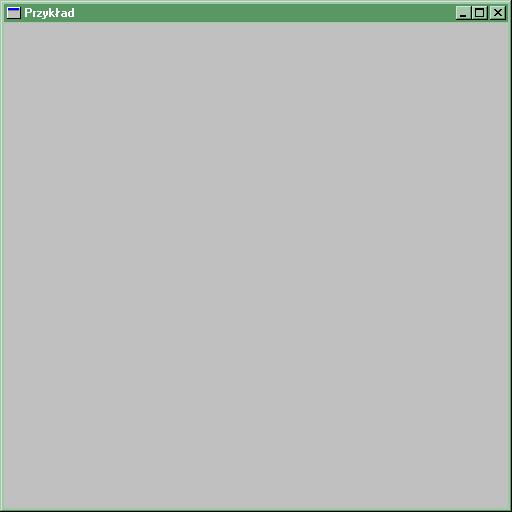
\includegraphics[width=0.5\textwidth]{./pic/p00}
\caption{Efekt działania pierwszego przykładowego programu}
\end{center}
\end{figure}

Z punktu widzenia syntaktyki - jest to zwykły program w języku C. Być może rozczarowujące jest to, że
program ten jest aż tak długi. Okazuje się jednak, że prościej się po prostu nie da. Jeżeli w jakimkolwiek
innym języku programowania lub przy użyciu jakichś bibliotek da się napisać prostszy program 
tworzący okno (a jak zobaczmy w rozdziale \ref{netTworzenieOkien} analogiczny program w C\# 
zajmuje mniej więcej 10 linii kodu), będzie to zawsze oznaczało, że część kodu jest po prostu ukryta przed
programistą.

Z tego właśnie powodu mówimy, że interfejs Win32API jest "najbliżej" systemu operacyjnego jak tylko jest
to możliwe (czasem mówi się też, że jest on "najniższym" interfejsem programowania). Każda inna
biblioteka umożliwiająca tworzenie okien {\bf musi} korzystać z funkcji Win32API, opakowując je
ewentualnie w jakiś własny interfejs programowania. 

Wielu programistów znających bardzo dobrze Win32API uważa to za jego najwięszą zaletę. To właśnie bowiem
Win32API daje największą kontrolę nad tym jak wygląda okno i jak się zachowuje. 

Ale wróćmy do naszego programu. Pierwsza ważna różnica między 
programem Windowsowym a zwykłym programem w języku C, to brak funkcji
{\bf main}, zastąpionej przez {\bf WinMain}. Tradycyjnie funkcja ta ma następujący prototyp:

\begin{scriptsize}
\begin{verbatim}
int
WINAPI
WinMain(

    HINSTANCE hInstance,
    HINSTANCE hPrevInstance,
    LPSTR lpCmdLine,
    int nShowCmd
    );
\end{verbatim}
\end{scriptsize}

W tej deklaracji
\begin{itemize}
	
	\item {\bf WINAPI} oznacza konwencję przekazywania parametrów do funkcji. 
	Zwykle w którymś z plików nagłówkowych znajdziemy po prostu 
	{\bf \#define WINAPI \_\_stdcall}\footnote{O innych konwencjach przekazywania parametrów do fukcji
	({\bf \_stdcall, \_cdecl, \_pascal}) warto poczytać, ponieważ niezgodność konwencji bywa źródłem
	problemów przy łączeniu bibliotek napisanych w różnych językach, np. Delphi i Visual Basicu.}
	\item {\bf hInstance}, jak sugeruje typ, jest uchwytem. W tym przypadku jest to uchwyt
	do bieżącej instancji aplikacji.

	\item {\bf hPrevInstance} to uchwyt do poprzedniej instancji tej aplikacji. W Win16API 
	za pomocą tego uchwytu można było zidentyfikować istniejącą już w systemie instancję aplikacji
	i uaktywnić ją w razie potrzeby. W Win32API ten parametr jest zawsze równy NULL i zachowano go
	tylko ze względów historycznych. Do identyfikowania innych instancji aplikacji w Win32API należy
	użyć jakichś trwałych obiektów, na przykład {\bf Mutexów}\footnote{Więcej o Mutexach 
	na stronie~\pageref{subsection_mutexy}}.

	\item {\bf lpCmdLine} to lista parametrów programu. W programie Windowsowym, w przeciwieństwie
	do zwykłego programu w języku C, wszystkie parametry przekazywane są w tej jednej tablicy. 
	Oznacza to, że programista musi sam zatroszczyć się o wyłowienie kolejnych parametrów z listy.
	Inaczej też niż w zwykłym programie w C można uzyskać informację o lokalizacji bieżącej
	aplikacji w systemie plików: zamiast odczytać zerowy parametr na liście parametrów,
	programista woła funkcję API {\bf GetModuleFileName}.

	\item Windows może aktywować okno na różne sposoby, m.in.:

	\begin{itemize}
		\item SW\_HIDE, ukrywa okno
		\item SW\_MINIMIZE, okno jest zminimalizowane
		\item SW\_RESTORE, SW\_SHOWNORMAL, aktywuje okno w jego oryginalnych rozmiarach
		\item SW\_SHOW, aktywuje okno w jego bieżących rozmiarach
		\item SW\_SHOWMAXIMIZED, okno jest zmaksymalizowane
	\end{itemize}
	{\bf nShowCmd} sugeruje aplikacji sposób pokazania głównego okna. Programista
	może oczywiście tę informację zlekceważyć, jednak nie jest to dobrą praktyką.

\end{itemize}

Druga ważna różnica różnica między programem Windowsowym a zwykłym programem w języku C, 
to mnóstwo nowych funkcji i struktur od jakich roi się w programie Windowsowym. Zauważmy, że samo
utworzenie okna jest procesem o tyle skomplikowanym, że wymaga wcześniej utworzenia tzw.{\em klasy okna}.
Chodzi o to, by wszystkie okna o podobnych właściwościach mogły mieć tę samą funkcję obsługi komunikatów
(o komunikatach za chwilę). 
Na przykład wszystkie przyciski są okami utworzonymi na bazie klasy {\bf BUTTON}, 
wskazującej na odpowiednią funkcję
obsługi zachowań przycisku. Aplikacja może tworzyć dowolną ilość okien bazujących na tej samej klasie, 
za każdym razem konkretyzując pewne dodatkowe cechy każdego nowego okna.

Aby zarejestrować w systemie nową klasę okna należy skorzystać z funkcji 

\begin{scriptsize}
\begin{verbatim}
ATOM RegisterClassEx(

    CONST WNDCLASSEX *lpwcx	
   );
\end{verbatim}
\end{scriptsize}

Klasa okna utworzona przez aplikację jest automatycznie wyrejestrowywania przy zakończeniu
aplikacji. Okna tworzy się za pomocą funkcji 

\begin{scriptsize}
\begin{verbatim}
HWND CreateWindowEx(

    DWORD dwExStyle,	// rozszerzony styl okna
    LPCTSTR lpClassName,	// nazwa klasy okna
    LPCTSTR lpWindowName,	// nazwa okna
    DWORD dwStyle,	// styl okna
    int x,	// pozycja okna
    int y,	
    int nWidth,	// szerokość
    int nHeight,	// wysokość
    HWND hWndParent,	// uchwyt okna macierzystego
    HMENU hMenu,	// uchwyt menu lub identyfikator okna potomnego
    HINSTANCE hInstance,	// instancja aplikacji
    LPVOID lpParam 	
   )
\end{verbatim}
\end{scriptsize}

Zapamiętajmy przy okazji prawidłowość: wiele funkcji API istnieje w dwóch wariantach,
podstawowym i rozszerzonym. Bardzo często funkcje podstawowe oczekują pewnej ściśle określonej ilości 
parametrów, natomiast funkcje rozszerzone oczekują jednego parametru, którym jest struktura z 
odpowiednio wypełnionymi polami\footnote{Nie jest to jednak regułą}. 

\subsection{Komunikaty}

W przykładzie z poprzedniego rozdziału widzieliśmy, że funkcja obsługi okna zajmuje się obsługą
komunikatów docierających do okna. Komunikaty pełnią w systemie Windows główną rolę jako środek
komunikacji między różnymi obiektami. Jeżeli gdziekolwiek w systemie dzieje się coś, co wymaga
poinformowania jakiegoś innego obiektu, najprawdopodobniej ta informacja przepłynie w postaci
komunikatu.

Obsługą komunikatów, ich rozdzielaniem do odpowiednich obiektów zajmuje się jądro systemu. 
W praktyce każde okno ma swoją własną {\em kolejkę komunikatów},
w której system umieszcza kolejne komunikaty, które mają swoje źródło gdzieś w systemie, a ich
przeznaczeniem jest dane okno. 

Programista może kazać oknu przechwytywać odpowiednie komunikaty, może również inicjować komunikaty
i kierować je do wybranych okien. W funkcji obsługi komunikatów programista sam decyduje o tym, na które
komunikaty okno powinno reagować. Najczęściej są to komunikaty typowe. Programista nie ma obowiązku reagować
na wszystkie możliwe komunikaty.

\begin{table}[ht]
	\begin{center}

	\mbox{$\ldots$}             \\ 
	\framebox[4cm]{Komunikat X}  \\ 
	\framebox[4cm]{Komunikat Y}  \\ 
	\framebox[4cm]{Komunikat Z}  \\ 
	 $\downarrow$                \\
	\framebox[7cm]{Okno}  
	\end{center}
\caption{Z każdym oknem system kojarzy kolejkę komunikatów dla niego przeznaczonych} 
\end{table}

Oto lista ważniejszych komunikatów, jakie mogą docierać do okna.

\begin{description}
\item[WM\_CHAR] Dociera do aktywnego okna po tym, jak komunikat WM\_KEYDOWN zostanie przetłumaczony
	w funkcji TranslateMessage().

        \begin{description}
		\item[chCharCode = (TCHAR) wParam;] Znakowy kod wciśniętego klawisza.
		\item[lKeyData = lParam;] Ilość powtórzeń, kody rozszerzone.
	\end{description}

\item[WM\_CLOSE] Dociera do aktywnego okna przed jego zamknięciem. Jest to chwila kiedy można
	jeszcze anulować zamknięcie okna.

\item[WM\_COMMAND] Dociera do aktywnego okna przy wyborze pozycji z menu lub jako powiadomienie
	od okna potomnego.

        \begin{description}
		\item[wNotifyCode = HIWORD(wParam);] Kod powiadomienia.
		\item[wID = LOWORD(wParam);] Identyfikator pozycja menu lub okna potomnego.
		\item[hwndCtl = (HWND) lParam;] Uchwyt okna potomnego.
	\end{description}

\item[WM\_CREATE] Dociera do okna po jego utworzeniu za pomocą CreateWindow() ale przed jego
        pierwszym pojawieniem się. Jest zwykle wykorzystywany na tworzenie okien potomnych,
	inicjowanie menu czy inicjowanie podsystemów OpenGL, DirectX itp.

        \begin{description}
		\item[lpcs = (LPCREATESTRUCT) lParam;] Informacje o utworzonym oknie.
	\end{description}

	\begin{scriptsize}
	\begin{verbatim}
	typedef struct tagCREATESTRUCT { // cs 
	    LPVOID    lpCreateParams; 
	    HINSTANCE hInstance; 
	    HMENU     hMenu; 
	    HWND      hwndParent; 
	    int       cy; 
	    int       cx; 
	    int       y; 
	    int       x; 
	    LONG      style; 
	    LPCTSTR   lpszName; 
	    LPCTSTR   lpszClass; 
	    DWORD     dwExStyle; 
	} CREATESTRUCT; 
	\end{verbatim}
	\end{scriptsize}

\item[WM\_KEYDOWN] Dociera do aktywnego okna gdy zostanie naciśnięty klawisz {\em nie}systemowy (czyli
	dowolny klawisz bez wciśniętego klawisza ALT).

        \begin{description}
		\item[nVirtKey = (int) wParam;] Kod klawisza.
		\item[lKeyData = lParam;] Ilość powtórzeń, kody rozszerzone.
	\end{description}

\item[WM\_KEYUP] Dociera do aktywnego okna gdy zostanie zwolniony klawisz {\em nie}systemowy (czyli
	dowolny klawisz bez wciśniętego klawisza ALT).

        \begin{description}
		\item[nVirtKey = (int) wParam;] Kod klawisza.
		\item[lKeyData = lParam;] Ilość powtórzeń, kody rozszerzone.
	\end{description}

\item[WM\_KILLFOCUS] Dociera do aktywnego okna przed przekazaniem aktywności innemu oknu.

        \begin{description}
		\item[hwndGetFocus = (HWND) wParam;] Uchwyt okna, ktróre stanie się aktywne.
		\item[lKeyData = lParam;] Ilość powtórzeń, kody rozszerzone.
	\end{description}

\item[WM\_LBUTTONDBLCLK] Dociera do aktywnego okna gdy jego obszar zostanie dwukliknięty.

        \begin{description}
		\item[fwKeys = wParam;] Informuje o tym, czy jednocześnie są wciśnięte klawisze systemowe: SHIFT, CTRL.
		\item[xPos = LOWORD(lParam);] Współrzędna X dwuklikniętego punktu względem punktu w lewym górnym
			rogu obszaru klienckiego okna.
		\item[yPos = HIWORD(lParam);] Współrzędna Y dwuklikniętego punktu względem punktu w lewym górnym
			rogu obszaru klienckiego okna.
	\end{description}

\item[WM\_LBUTTONDOWN] Dociera do aktywnego okna gdy jego obszar zostanie kliknięty za pomocą lewego przycisku.

        \begin{description}
		\item[fwKeys = wParam;] Informuje o tym, czy jednocześnie są wciśnięte klawisze systemowe: SHIFT, CTRL.
		\item[xPos = LOWORD(lParam);] Współrzędna X dwuklikniętego punktu względem punktu w lewym górnym
			rogu obszaru klienckiego okna.
		\item[yPos = HIWORD(lParam);] Współrzędna Y dwuklikniętego punktu względem punktu w lewym górnym
			rogu obszaru klienckiego okna.
	\end{description}

\item[WM\_LBUTTONUP] Dociera do aktywnego okna gdy użytkownik zwalna lewy przycisk myszy, a wskaźnik znajduje
		się nad obszarem klienckim okna.

        \begin{description}
		\item[fwKeys = wParam;] Informuje o tym, czy jednocześnie są wciśnięte klawisze systemowe: SHIFT, CTRL.
		\item[xPos = LOWORD(lParam);] Współrzędna X dwuklikniętego punktu względem punktu w lewym górnym
			rogu obszaru klienckiego okna.
		\item[yPos = HIWORD(lParam);] Współrzędna Y dwuklikniętego punktu względem punktu w lewym górnym
			rogu obszaru klienckiego okna.
	\end{description}

\item[WM\_MOVE] Dociera do okna po tym jak zmieniło się jego położenie.

        \begin{description}
		\item[xPos = LOWORD(lParam);] Nowa współrzędna X okna.
		\item[yPos = HIWORD(lParam);] Nowa współrzędna Y okna.
	\end{description}

\item[WM\_PAINT] Dociera do okna gdy jego obszar kliencki wymaga odrysowania. Więcej o tym
		komunikacie na stronie~\pageref{subsection_gdi}.

\item[WM\_SIZE] Dociera do okna, gdy zmienił się jego rozmiar.

        \begin{description}
		\item[nWidth = LOWORD(lParam);] Nowa szerokość okna.
		\item[nHeight = HIWORD(lParam);] Nowa wysokość okna.
	\end{description}

\item[WM\_QUIT] Powoduje zakończenie pętli komunikatów i tym samym zakończenie aplikacji.

        \begin{description}
		\item[nExitCode = (int) wParam;] Kod zakończenia.
	\end{description}

\item[WM\_SYSCOLORCHANGE] Dociera do wszystkich okien po tym, gdy zmienią się ustawienia kolorów pulpitu.

\item[WM\_TIMER] Dociera do aktywnego okna od ustawionego przez aplikację zegara. Więcej o zegarach 
		na stronie~\pageref{subsubsection_zegary}.

	\begin{description}
		\item[wTimerID = wParam;] Identyfikator zegara.
		\item[tmprc = (TIMERPROC *) lParam;] Adres funkcji obsługi zdarzenia.
	\end{description}
 
\item[WM\_USER] Pozwala użytkownikowy definiować własne komunikaty. Użytkownik tworzy komunikat
	za pomocą funkcji 

	\begin{scriptsize}
	\begin{verbatim}
	UINT RegisterWindowMessage(

	    LPCTSTR lpString 	
	   );	
	\end{verbatim}
	\end{scriptsize}

\end{description}

\label{apiPetlaObslugiKomunikatow}
Zaproponowana w przykładzie konstrukcja pętli obsługi komunikatów jest bardzo charakterystyczna.
\begin{scriptsize}
\begin{verbatim}
/* Pętla obsługi komunikatów */
while(GetMessage(&messages, NULL, 0, 0))
{
       /* Tłumacz kody rozszerzone */
       TranslateMessage(&messages);
       /* Obsłuż komunikat */
       DispatchMessage(&messages);
}
\end{verbatim}
\end{scriptsize}

Funkcja {\bf GetMessage} czeka na pojawienie się komunikatu w kolejce komunikatów, zaś
{\bf DispatchMessage} wysyła komunikat do funkcji obsługi komunikatów. 

Funkcja GetMessage jest jednak funkcją {\em blokującą}, to znaczy że wykonanie programu zostanie
wstrzymane na tak długo, aż jakaś wiadomość pojawi się w kolejce komunikatów okna aplikacji. 
Najczęściej aplikacja wstrzymywana jest na kilka czy kilkanaście milisekund, bowiem komunikaty 
napływają do okna dość często, oznacza to jednak, że część cennego czasu aplikacja marnuje
na biernym oczekiwaniu na komunikaty. 

Takie zachowanie nie byłoby wskazane dla aplikacji, która miałaby działać w sposób ciągły, na przykład
tworząc grafikę czy inne efekty w czasie rzeczywistym. Rozwiązaniem jest zastosowanie
innej postaci pętli obsługi komunikatów, alternatywnej dla pokazanej powyżej, wykorzystującej
nieblokującą funkcję {\bf PeekMessage}, która po prostu
sprawdza czy w kolejce komunikatów jest jakiś komunikat, a jeśli nie - oddaje sterowanie
do pętli obsługi komunikatów. Wybór pomiędzy oboma funkcjami (a co za tym idzie - między
dwoma możliwościami konstrukcji pętli obsługi komunikatów) należy do programisty.

\begin{scriptsize}
\begin{verbatim}
/* Pętla obsługi komunikatów */
while (TRUE)
{
     /* Sprawdź czy są jakieś komunikaty do obsłużenia */ 	
     if (PeekMessage (&msg, NULL, 0, 0, PM_REMOVE))
     {
          if (msg.message == WM_QUIT)
               break ;

          TranslateMessage (&msg) ;
          DispatchMessage (&msg) ;
     }
     else
     {
          // "czas wolny" aplikacji do wykorzystania do innych celów 
	  // niż obsługa komunikatów -
     }
}
\end{verbatim}
\end{scriptsize}
